\documentclass[12pt,letterpaper, onecolumn]{exam}
\usepackage{amsmath}
\usepackage{amssymb}
\usepackage{tikz}
\usepackage[lmargin=71pt, tmargin=1.2in]{geometry}  %For centering solution box
\lhead{\\}
\rhead{\\}
% \chead{\hline} % Un-comment to draw line below header
\thispagestyle{empty}   %For removing header/footer from page 1

\begin{document}

\begingroup  
    \centering
    \LARGE BIOSTAT 522A\\
    \LARGE Homework 2\\[0.5em]
    \large \today\\[0.5em]
    \large Jiangyue Wang\par
    \large jyuewang@uw.edu\par
    \large QERM, College of the Environment\par
\endgroup
\rule{\textwidth}{0.4pt}
\pointsdroppedatright   %Self-explanatory
\printanswers
\renewcommand{\solutiontitle}{\noindent\textbf{Ans:}\enspace}   %Replace "Ans:" with starting keyword in solution box
\begin{questions}
    \question Problem 1
    \begin{solution}
    Imagine we have a coin flipping process with $m(m>n)$ total trials, head will be regarded as success in a Bernoulli trial with a probability of $p$. Then, $P(Y>n)$ means that the $r^{th}$ success must have happened in the $i^{th} (n<i \leq m)$ trial. Thus, the number successes left for the first $n$ trials would be equal to or less than $r-1$. Here, $\leq r-1$ successes in $n$ trials can be translated to $P(X \leq r-1)$ when $X \sim Bin(n,p)$. As $X$ and $Y$ are discrete random variables with support in integers, $P(X \leq r-1) = P(X < r)$, so finally we have $P(X<r) = P(Y>n)$.
    \end{solution}

    \question Problem 2
    \begin{solution}
        \begin{enumerate}
            \item $p_X(x) = \frac{\binom{4}{x} \binom{4}{4-x}}{\binom{8}{4}} = \frac{288}{35(x!)^2((4-x)!)^2}, x=0,1,2,3,4$
            \item \begin{align*}
                p^* & = P(X \geq x^*), x^* \in \{0,1,2,3,4\} \\
                &\text{When $x^*$=4,} \\
                p^* & = P(X \geq 4) = P(X = 4) \\
                & = \frac{\binom{4}{4} \binom{4}{4-4}}{\binom{8}{4}} \\
                & = \frac{1}{70} = 0.0143
            \end{align*}
            This means that the probability with no supernatural abilities would attain as many or more correct answers is extremely low (1.43\%), so the lady's outcome is a rare event without superpower ability. Thus, I would be inclined to accept that the lady has supernatural power. \\
            \begin{align*}
              & \text{When $x^*$=3, as values of X are mutually exclusive,} \\
              p^* & = P(X \geq 3) = P(X = 4)+P(X = 3) \\
                & = \frac{\binom{4}{4} \binom{4}{4-4}}{\binom{8}{4}} + \frac{\binom{4}{3} \binom{4}{4-3}}{\binom{8}{4}} \\
                & = \frac{17}{70} = 0.243
            \end{align*}
            This means that the probability with no supernatural abilities would attain as many or more correct answers is relatively low but not very low (24.3\%, approximately one in four), so the lady's outcome is not a very rare event without superpower ability. Thus, I would be inclined to reject that the lady has supernatural power. \\
            \begin{align*}
              & \text{When $x^*=2$, as values of X are mutually exclusive,} \\
              p^* & = P(X \geq 2) = P(X = 4)+P(X = 3)+P(X = 2) \\
                & = \frac{\binom{4}{4} \binom{4}{4-4}}{\binom{8}{4}} + \frac{\binom{4}{3} \binom{4}{4-3}}{\binom{8}{4}} + \frac{\binom{4}{2} \binom{4}{4-2}}{\binom{8}{4}} \\
                & = \frac{53}{70} = 0.757
            \end{align*}
            This means that the probability with no supernatural abilities would attain as many or more correct answers is quite high (75.7\%), so the lady's outcome is a pretty common event without superpower ability. Thus, I would be inclined to reject that the lady has supernatural power. \\
            \item \begin{align*}
                p_X(x) & = \frac{\binom{m}{N-x} \binom{n}{x}}{\binom{m+n}{N}} \\
                & = \frac{m!n!N!(m+n-N)!}{(n-x)!(m-N+x)!x!(N-x)!(m+n)!}
            \end{align*}
            \item $N$ is the number of cups that the lady chooses, which is four; $n$ is the number of cups with milk added first, which is four; $m$ is the number of cups with tea added first, which is four; $x^*$ is the number of correct answers (i.e., the number of cups with milk added first that the lady chooses).
        \end{enumerate}
    \end{solution}

    \question Problem 3
    \begin{solution}
    \begin{enumerate}
        \item If $f$ is a density, then $\int_\mathcal{X} f(x)dx = 1$. Thus, 
        \begin{align*}
            \int_{\mathcal{X}} f(x)dx & = \int_{0}^{1} x^2dx + \int_{1}^{4} Cdx \\
            & = \frac{1}{3}x^3|_{0}^{1} + Cx|_{1}^{4} \\
            & = \frac{1}{3} + 3C = 1 \\
            \text{Thus, we have } C & = \frac{2}{9}.
        \end{align*}
        The graph of $f(x)$ is shown as the following:
        \begin{center}
        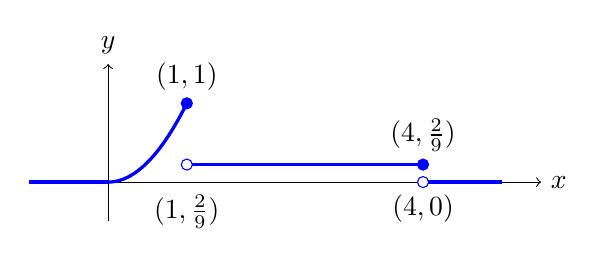
\begin{tikzpicture}
            \draw[->] (-1, 0) -- (5.5, 0) node[right] {$x$};
            \draw[->] (0, -0.5) -- (0, 1.5) node[above] {$y$};
            \draw[domain=-1:0, smooth, variable=\x, blue, very thick]  plot ({\x},{0});
            \draw[domain=0:1, smooth, variable=\x, blue, very thick] plot ({\x},{\x*\x});
            \draw[domain=1:4, smooth, variable=\x, blue, very thick]  plot ({\x},{2/9});
            \draw[domain=4:5, smooth, variable=\x, blue, very thick]  plot ({\x},{0});
            \filldraw[blue] (1,1) circle (2pt);
            \node[inner sep=1pt, label={90:{$(1,1)$}}] (a) at (1,1) {};
            \filldraw[color=blue, fill=blue!0] (1,2/9) circle (2pt);
            \node[inner sep=1pt, label={-90:{$(1,\frac{2}{9})$}}] (a) at (1,0) {};
            \filldraw[color=blue] (4,2/9) circle (2pt);
            \node[inner sep=1pt, label={90:{$(4,\frac{2}{9})$}}] (a) at (4,2/9) {};
            \filldraw[color=blue, fill=blue!0] (4,0) circle (2pt);
            \node[inner sep=1pt, label={-90:{$(4,0)$}}] (a) at (4,0) {};
        \end{tikzpicture}
        \end{center}

        \item For $x < 0$, $F_X(x) = P(X \leq x) = \int_{-\infty}^{x} f(x)dx = 0$. \\ 
        For $x\leq 1$, $F_X(x) = P(X \leq x) = \int_{-\infty}^{x} f(x)dx = \frac{1}{3}x^3$. \\
        For  $1 < x\leq 4$, $F_X(x) = P(X \leq x) = \int_{-\infty}^{1} f(x)dx + \int_{1}^{x} f(x)dx  = \frac{1}{3} + \frac{2}{9}(x-1) = \frac{2}{9}x + \frac{1}{9}$. \\
        For $x > 4$, $F_X(x) = P(X \leq x) = \int_{-\infty}^{1} f(x)dx + \int_{1}^{4} f(x)dx + \int_{4}{\infty} f(x)dx  = \frac{1}{3} + \frac{2}{3} + 0 = 1$. \\
        Thus, we have \\
        $$F_X(x) = \left \{
            \begin{array}{rcl}
                0  &\mbox{for} & x<0 \\ 
                \frac{1}{3}{x^3} & \mbox{for} & 0 \leq x \leq 1 \\
                \frac{2}{9}x + \frac{1}{9} & \mbox{for} & 1 < x \leq 4 \\
                1 & \mbox{for} & x>4
            \end{array} \right $$
        \begin{center}
        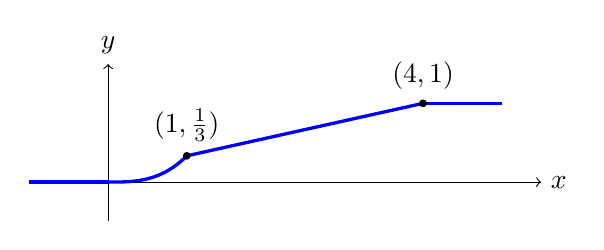
\begin{tikzpicture}
            
            \draw[->] (-1, 0) -- (5.5, 0) node[right] {$x$};
            \draw[->] (0, -0.5) -- (0, 1.5) node[above] {$y$};
            \draw[domain=-1:0, smooth, variable=\x, blue, very thick]  plot ({\x},{0});
            \draw[domain=0:1, smooth, variable=\x, blue, very thick] plot ({\x},{\x*\x*\x*1/3});
            \draw[domain=1:4, smooth, variable=\x, blue, very thick]  plot ({\x},{2/9*\x+1/9});
            \draw[domain=4:5, smooth, variable=\x, blue, very thick]  plot ({\x},{1});

            \node[circle, fill, inner sep=1pt, label={90:{$(1,\frac{1}{3})$}}] (a) at (1,1/3) {};
            \node[circle, fill, inner sep=1pt, label={90:{$(4,1)$}}] (a) at (4,1) {};
        \end{tikzpicture}
        \end{center}
    \item $P(|X-2|<1.5) = P(0.5<X<3.5) = F(3.5) - F(0.5) = \frac{2}{9} \times 3.5 + \frac{1}{9} - \frac{1}{3} \times 0.5^3 = \frac{61}{72} = 0.847$
    \item The derivative of $F(x)$ exists for $x\in (-\infty,1) \cup (1,4) \cup (4, \infty)$ for all x. But if we are talking about the support of $x$, then it only exists for $x\in (0,1) \cup (1,4)$. When the derivative does not exist, \\
    $$f(x) = \left \{
            \begin{array}{rcl}
                1 & \mbox{for} & x=1 \\
                \frac{2}{9} & \mbox{for} & x=4
            \end{array} \right $$
    \item
    \begin{align*}
        E(X) & = \int_{0}^{4} xf(x)dx \\
        & = \int_{0}^{1} x^3dx + \int_{1}^{4} \farc{2}{9}xdx \\
        & = \frac{23}{12} = 1.917
    \end{align*}
    \begin{align*}
        E(X^2) & = \int_{0}^{4} x^2f(x)dx \\
        & = \int_{0}^{1} x^4dx + \int_{1}^{4} \farc{2}{9}x^2dx \\
        & = \frac{73}{15} = 4.867 \\
        Var(X) & = E(X^2) - (E(X))^2 \\
        & = \frac{859}{720} = 1.193
    \end{align*}
    
    \end{enumerate}
    \end{solution}

    \question Problem 4
    \begin{solution}
        \begin{enumerate}
            \item $N$ is this game can be considered as a random variable that follows geometric distribution, and heads can be considered as success (i.e., $N \thicksim Geo(p)$, where $p = 0.5$). \\
        Thus, $E(N) = \frac{n}{p} = \frac{1}{0.5} = 2$, $2^{E(N)} = 4$. \\
            \item Let $g(N) = 2^N$, so now we are calculating $E(g(N))$. \\
            \begin{align*}
                E(g(N)) & = \sum_{N=1}^\infty g(N)f_N(N) \\
                & = \sum_{N=1}^\infty 2^N*(1-p)^{N-1}*p \\
                & = \sum_{N=1}^\infty 2^N*0.5^{N-1}*0.5 \\
                & = \sum_{N=1}^\infty 2^N*0.5^{N} \\
                & = \sum_{N=1}^\infty 1^N \\
                & = \infty
            \end{align*}
            \item The fair price is then $E(2^N)$, which is infinity, so the fair price in the long term does not exist.
        \end{enumerate}
        
    \end{solution}

    \question Problem 5
    \begin{solution}
        \begin{enumerate}
            \item Let $Y = aX+b$, $E(Y) = aE(X)+b$. 
            \begin{align*}
                E(Y^2) & = E((aX+b)^2) \\
                & = E(a^2X^2 + 2abX + b^2) \\
                & = a^2E(X^2)+2abE(X)+b^2 \\
                Var(Y) & = E(Y^2) - E(Y)^2 \\
                & = a^2E(X^2)+2abE(X)+b^2 - (aE(X) + b)^2 \\
                & = a^2E(X^2) - a^2E(X)^2 \\
                & = a^2Var(X)
            \end{align*}
            \item Let $W = \frac{X-\mu}{\sigma}$,
            \begin{align*}
                E((X-E(X))^{2j}) & = E((X-\mu)^{2j}) \\
                & = E((\sigma W)^{2j}) \\
                & = \sigma^{2j} E(W^{2j}) \\
                & = \sigma^{2j} (\frac{1}{2})^j\frac{(2j)!}{j!} \\
                & = \sigma^{2j} (2j-1)!! \\
            \end{align*}
            \item Let $U \thicksim Gamma(\alpha, \beta)$, $M_U(t) = (1-\beta t)^{-\alpha}$ $(t<\frac{1}{\beta})$. \\
            \begin{align*}
                M_Y(t) & = \prod_{i=1}^n M_{X_i}(t), t<\frac{1}{\beta} \\
                & = \prod_{i=1}^n (1-\beta t)^{-\alpha _i}, t<\frac{1}{\beta} \\
                & = (1-\beta t)^{-\sum_{i=1}^n \alpha _i}, t<\frac{1}{\beta} \\
                & = (1-\beta t)^{-\alpha}, t<\frac{1}{\beta} \\
                & = M_U(t)
            \end{align*}
            Thus, $Y$ has the same distribution with $U$, that is $Gamma(\alpha, \beta)$.
            \begin{align*}
                M_W(t) & = \prod_{i=1}^n M_{Z_i}(t), t<\frac{1}{\beta}\\
                & = \prod_{i=1}^n (1-\beta_i t)^{-\alpha}, t<\frac{1}{\beta} \\
                M_U(t) & = (1-\beta t)^{-\alpha}, t<\frac{1}{\beta} \\
                & = (1-\sum_{i=1}^n \beta_i t)^{-\alpha}, t<\frac{1}{\beta}\\
                & \neq M_W(t)\\
            \end{align*}
            Thus, $W$ does not have the same distribution with $U$.
        \end{enumerate}
    \end{solution}
    \question Problem 6
    \begin{solution}
        \begin{enumerate}
            \item $$p_X(x) = \left \{
            \begin{array}{rcl}
                p+(1-p)e^{-\lambda}  &\mbox{for} & x=0 \\ 
                (1-p)\frac{e^{-\lambda}(\lambda)^x}{x!} & \mbox{for} & x=1,2,3,...... \\
            \end{array} \right $$
            \item $Bernoulli(p)$ means that the probability of success (get a value of 1) is $p$. While in zero-inflated Poisson distribution, $p$ is the probability of getting a value of 0. Thus, we should have a reversed Bernoulli distribution $1-I~Bernoulli(1-p)$ meaning whether we observe a structural 0. \\
            If $I = 1$, then $X=0$ (structural 0). If $I=0$, then $X$ is drawn from a Poisson distribution. Thus, $X$ can be represented by $(1-I)Y$, where $(1-I)$ determines whether we get a structural 0, and $Y$ follows a Poisson distribution with non-structural outcomes.
            \item Considering the theorem on product of the expectation of two independent random variables, $$E(X) = E(1-I)E(Y) = \lambda (1-p)$$
            \begin{align*}
                Var((1-I)Y) & = E(((1-I)Y)^2) - (E((1-I)Y))^2 \\
                & = E((1-I)^2)E(Y^2)-(E((1-I)Y))^2 \\
                & = (Var(1-I)+E(1-I)^2)(Var(Y)+E(Y)^2)-(E((1-I)Y))^2 \\
                & = (p(1-p) +  (1-p)^2)(\lambda + \lambda^2)-(1-p)^2\lambda^2 \\
                & = (1-p)\lambda(1+\lambda p)
            \end{align*}
        \end{enumerate}
    \end{solution}
\end{questions}
\end{document}